%%%%%%%%%%%%%%%%%%%%%%%%%%%%%%%%%%%%%%%%%
% Simple Sectioned Essay Template
% LaTeX Template
%
% This template has been downloaded from:
% http://www.latextemplates.com
%
% Note:
% The \lipsum[#] commands throughout this template generate dummy text
% to fill the template out. These commands should all be removed when 
% writing essay content.
%
%%%%%%%%%%%%%%%%%%%%%%%%%%%%%%%%%%%%%%%%%

%----------------------------------------------------------------------------------------
% PACKAGES AND OTHER DOCUMENT CONFIGURATIONS
%----------------------------------------------------------------------------------------

\documentclass[12pt]{article} % Default font size is 12pt, it can be changed here
\usepackage[utf8]{inputenc} % utf8 support
\usepackage[T1]{fontenc}

\usepackage{geometry} % Required to change the page size to A4
\geometry{a4paper} % Set the page size to be A4 as opposed to the default US Letter

\usepackage{graphicx} % Required for including pictures

% \usepackage{float} % Allows putting an [H] in \begin{figure} to specify the exact location of the figure
\usepackage{wrapfig} % Allows in-line images such as the example fish picture

\usepackage[style=numeric, backend=biber, sorting=none]{biblatex}
\bibliography{kilgarvan.bib}

\linespread{1.2} % Line spacing

%\setlength\parindent{0pt} % Uncomment to remove all indentation from paragraphs

\graphicspath{{./img/}} % Specifies the directory where pictures are stored

\newlength{\wideitemsep}
\setlength{\wideitemsep}{.5\itemsep}
\addtolength{\wideitemsep}{-7pt}
\let\olditem\item
\renewcommand{\item}{\setlength{\itemsep}{\wideitemsep}\olditem}

\begin{document}

%----------------------------------------------------------------------------------------
% TITLE PAGE
%----------------------------------------------------------------------------------------

\begin{titlepage}
  \newcommand{\HRule}{\rule{\linewidth}{0.5mm}} % Defines a new command for the horizontal lines, change thickness here

  \center % Center everything on the page

  \textsc{\LARGE University College Cork}\\[1.5cm] % Name of your university/college
  \textsc{\Large Wind Energy}\\[0.5cm] % Major heading such as course name
  % \textsc{\large Minor Heading}\\[0.5cm] % Minor heading such as course title

  \HRule \\[0.4cm]
  { \huge Kilgarvan Wind Farm Visit 28-10-2015}\\[0.5cm] % Title of your document
  \HRule \\[1.5cm]

  \begin{minipage}{0.4\textwidth}
  \begin{flushleft} \large
  \emph{Author:} Peter \textsc{Armstrong} \\% Your name 
  \emph{Student ID:} 115224113
  \end{flushleft}
  \end{minipage}
  ~
  \begin{minipage}{0.4\textwidth}
  \begin{flushright} \large
  % \emph{Supervisor:} \\
  % Dr. James \textsc{Smith} % Supervisor's Name
  \end{flushright}
  \end{minipage}\\[4cm]

  {\large \today}\\[3cm] % Date, change the \today to a set date if you want to be precise

  \vfill % Fill the rest of the page with whitespace

% itemize changes
\newlength{\wideitemsep}
\setlength{\wideitemsep}{.5\itemsep}
\addtolength{\wideitemsep}{-7pt}
\let\olditem\item
\renewcommand{\item}{\setlength{\itemsep}{\wideitemsep}\olditem}

\end{titlepage}

%----------------------------------------------------------------------------------------
% TABLE OF CONTENTS
%----------------------------------------------------------------------------------------

% \tableofcontents % Include a table of contents

% \newpage % Begins the essay on a new page instead of on the same page as the table of contents 

%----------------------------------------------------------------------------------------
% INTRODUCTION
%----------------------------------------------------------------------------------------

\section{Site Description} % Major section

The Kilgarvan wind farms are situated on the western side of the Derrynasaggart mountains, Co. Kerry. In the area, there is a cluster of five wind farms. This group of wind farms have been built over the last 10 years.

  \begin{center}
    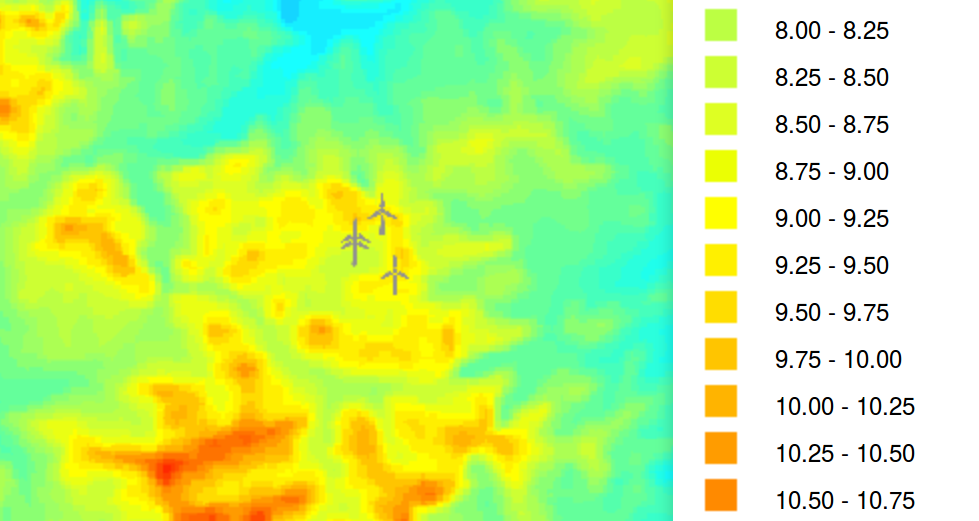
\includegraphics[width=1\textwidth]{seai_wind_atlas_kilgarvan}
  \end{center}
  \caption{Wind speed at 75m - SEAI Wind Atlas - Kilgarvan Area}

According to the SEAI Wind Atlas \cite{seai_atlas}, the area has average wind speeds at 75m height of 8 - 10 ms^-1.

% TODO: Something about wind reliability - weibull

The terrain is flat/not flat - based on what criteria.


\subsection{Access Route}
Access to Kilgarvan windfarm is off the N22. 

The first bit of electricity infrastructure visible is an Eirgrid/ESB operated substation just off the main road. This substation connects directly to the 110kV grid.

The wind farms are situated on the western side of the Derrynasaggart mountains. An access road winds from the Nxxx to the site. The road passes through both rocky and bog areas. Some cutting away of bog and rock was necessary to build the road. The road has a gentle incline and wide turns. Turbines were transported to the site in large sections on this road so it has a gentle incline and wide turns.
% reference for transporting turbine sections
The area on the lee side of the hills is forested. Although the land is owned by the wind farm operator, Brookfield, the forestry is managed by Caoilte.


% research building roads through bogs



\section{Technology Description}
\subsection{Electrical Grid}


\section{Operations and Conditions}

\subsection{A day in the life of a wind farmer}

\subsection{The day we visited}

\section{Conclusion}
Wind farming is a business.
Successful, large companies investing in it.


%----------------------------------------------------------------------------------------
% BIBLIOGRAPHY
%----------------------------------------------------------------------------------------
\printbibliography

%----------------------------------------------------------------------------------------

\end{document}